
\documentclass[10pt,a4paper,titlepage]{article}
\usepackage[english]{babel}
\usepackage[utf8]{inputenc}
\usepackage[margin=100pt]{geometry}
    
    
\usepackage{graphicx}   % Import pictures
%\usepackage{ragged2e}   % fullfill paragraphs
%\usepackage{multicol}
%\usepackage{xcolor}
%\usepackage{courier}
\usepackage{caption}
    
\usepackage[backend=biber, sorting=none]{biblatex}
\addbibresource{manual.bib}
    
    
    
\begin{document}
    
    %-----------------------------------------%
    %	            TITLE PAGE                %
    %-----------------------------------------%
    \begin{titlepage}
    \begin{center}
        % Headings
        \textsc{\LARGE Brno University of technology}\\[0.5cm]
        \textsc{\large Faculty of Information Technology}\\[8cm]
    
        % Title - lines
        { \huge \bfseries Monitoring and Generating Tools of Simple Distance-Vector Protocols}\\[0.3cm]
        { \Large \bfseries Project documentation}\\[0.5cm]
        { \bfseries Martin Benes}\\
    
    \end{center} 
    \end{titlepage}
    
    \newpage
    
    %-----------------------------------------%
    %	             DOCUMENT                 %
    %-----------------------------------------%
    \pagenumbering{gobble}
    
    \section*{RIP}
        %The task of the project was to gather informations about RIP protocols, RIPv1, RIPv2 and RIPng and
        %to write two programs in C, one of them RIP sniffer and the other RIP fake responder.

        \subsection*{Motivation}
            Internet. It is everywhere nowadays - it helps us order pizza, find a taxi, do shopping,
            connect us with all our friends but it also controls the lights, air condition units etc;
            it has become significant part of our lives. There is a lot of data flowing through each
            its part in every moment. This dataflow is directed ({\it routed}) by devices called routers,
            knots in the huge network.

            \begin{figure}[h!]
                \begin{center}
                    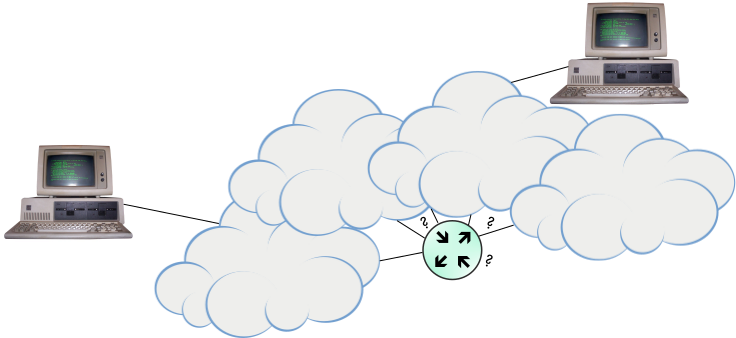
\includegraphics[width=0.80\textwidth]{routing.png}
                    \caption{ Routing. \label{fig:routing}}
                \end{center}
            \end{figure}

            Each router has multiple routes connected to it and it has a single task: it recieves
            a chunk of data (packet) with an address on it and it is supposed to send it closer to
            the target device in the network as you can see in the picture \ref{fig:routing}.
            The router must decide which route should the packet go. And this is exactly what the
            RIP protocol does. 
    
        \subsection*{RIP Protocol}
            {\it Routing Information Protocol} is a routing protocol. It enables routers to communicate and to react
            on the network topology changes. RIP is a distance-vector protocol - no router knows the whole structure
            of the network. The method it uses to count the shortest path is Bellman-Ford algorithm. A hop count
            is used as a path cost.

            \paragraph{Communication}
            The protocol uses UDP transport protocol and it has registered port 520 (RIPv1, RIPv2) and 521 (RIPng).
            Two basic types of messages are used, RIP Request and RIP Response.

            {\it RIP Request} is sent when the router asks other router for the routing table content (all or just a part).

            {\it RIP Response} includes the routing table of the sender. The destination port is the port in the Source Port
            array in the RIP Request. But it can be sent even without previous RIP Request received.\cite{RIPngStd}

        \subsection*{RIP Route Determination}
            Three main items of each record in the routing table are adress of the network/station, distance (hops)
            and interface. RIP protocol enables routers to share their routing tables and make sending of data through
            the network much more efficient. The receiving router always compares the new information with the one he has.

            If the network X is reachable in N+1 hops (router increases the number by one), it is compared with the content
            of the routing table. If the new route is better, it is set and algorithm is propagated to the neighbors to
            recalculate - this is done again again until the algorithm reaches convergence.\cite{RIPguide}

        \subsection*{Timeouts}

        \subsection*{RIP Problems}
            The popularity of the protocol is caused by its simplicity. Although it has some issues which led into replacing
            RIP protocol in different routing protocols (EIGTP, OSPF).

        \paragraph{Slow Convergence}
            Due to the fact that timeout for sending RIP Response is set by RFC to 30~s, convergence of the whole algorithm
            might take minutes, which is ages for today networing. The propagation of failure is even 180~s, initial delay
            for propagation.

        \paragraph{Loops}
            At special occasions routing loops may occur.

        \paragraph{Max hop count}
            The max hop count is limited to 15. Hop count 16 means unreachable network (distance infinity).

        \paragraph{CIDR unsupported}
            The first version of protocol was not designed for classless addresses; Therefore in modern networks is useless.
            It was fixed in RIPv2.

        \paragraph{IPv6 unsupported}
            Both RIPv1 and RIPv2 can work only with IPv4 addresses. The IPv6 addresses were enabled in RIPng.

    \subsection*{Versions of RIP}
        \paragraph{RIPv1}
        \paragraph{RIPv2}
        \paragraph{RIPng}


    




    
\section*{Implementation}
    
    \subsection*{Network}
    \begin{figure}[h!]
        \begin{center}
    %        \includegraphics[width=0.7\textwidth]{network.png}
            \caption{ Test network. \label{fig:network} \cite{laptop}}
        \end{center}
    \end{figure}
    The used test network was my personal home network. It consists of wireless
    devices, connected to the wireless router, which contains access point and DHCP agent.
    There is no protection like port security or DHCP snooping done.
    
    The router is then connected to the internet, and wireless devices, like my laptop
    or mobile are able to connect the internet indirectly through the AP.
    
    \subsection*{Program}
    
    The program was done in C, some tools were taken from C++. It implements the attack,
    where a DHCP Discovery packets are generated with random MAC in the DHCP header,
    but with real MAC is used in the link layer.
    
    Firstly, I wanted to do the program using raw socket. This would be needed, if 
    I would want to generate packets with random MAC address in Ethernet header as well.
    Then it came to me, that they do not have to be needed afterall. I rewrote the
    program and ended up with one third of a length of the code, but a fully functional.
    
    \begin{figure}[h!]
        \begin{center}
            %\includegraphics[width=0.5\textwidth]{ifconfig.png}
            \caption{ Network adapter configuration. \label{fig:ifconfig}}
        \end{center}
    \end{figure}
    
    \begin{figure}[h!]
        \begin{center}
            %\includegraphics[width=0.5\textwidth]{run.png}
            \caption{ Run command. \label{fig:run}}
        \end{center}
    \end{figure}
    
    
    \subsection*{Testing}
    For the testing, I used Wireshark to watch the network traffic. I attach a
    screenshot of testing procedure.
    
    When the program starts, every sent DHCP Discovery packet is followed by DHCP Offer
    packet. After sending a specific count of packets, there is no coming DHCP
    Offer whatsoever.
    
    The addresses starts with 10.0.2.16. Then they are offered one-by-one sequentially,
    ending with 10.0.2.30. More coming offers with a local IP address are not
    received.
    
    \begin{figure}[h!]
        \begin{center}
            %\includegraphics[width=1\textwidth]{wireshark.png}
            \caption{ Network traffic during atack. \label{fig:wireshark}}
        \end{center}
    \end{figure}
    
    \newpage
    \printbibliography
    
    \end{document}